\chapter{Language Design of \lang} \label{ch:language_design}
% Forklar hvordan vi løser problemet fra problemstillingen ovenover, og hvordan vores program generelt skal designes.

This chapter aims to explore the theoretical foundations and practical considerations involved in designing the \lang programming language. This chapter will provide a comprehensive analysis of the various aspects of language design. It will include the language criteria that guide the design process, the requirements that must be considered, and the syntax design, which includes Context-Free Grammars (CFGs) and Extended Backus-Naur Form (EBNF). Additionally, we will examine the static semantics of programming languages, including Abstract Syntax Trees (ASTs), scope rules, type rules and operational semantics. \\


\section{Language Criteria}\label{languageCriteriaForLang}
To begin, we will discuss the language criteria for \lang that serve as the guiding principles for designing a programming language. These criteria include readability, writability, and reliability. Each of these criteria will be explored in detail. Benefits and trade-offs associated with each will be discussed in relation to \lang.

\subsection{Readability} \label{Lang Readability}
Based on the analysis of existing programming languages in section \ref{ComparingLanguages}, high readability is important when designing a language aimed towards beginner programmers. This readability can be achieved by constructing a syntax that relates to concepts and terminology that beginner programmers are already familiar with from their education. Based on our own experiences, having a readable syntax that relates to known concepts, makes the language syntax more memorable, making the programming concepts easier to grasp and relate to.\\  

As stated in the analysis in section \ref{ComparingLanguages}, both Scratch and Quorum have high simplicity and use concepts and terminology related to the English language. Quorum focuses on readability over writability whereas Python does not. As \lang should help beginner programmers with transitioning to some common industry standards, \lang has been placed between Python and Quorum, but closer to Quorum on the scale in figure \ref{LD:readability_scale}. This is due to the focus on readability, as people who have not programmed before, should be able to better recognize the constructs of \lang. But since \lang should be related to common industry languages, constructs such as statement terminators, and scope declaration should be equivalent to these languages.\\  

\begin{figure}[H] 
    \begin{center}
        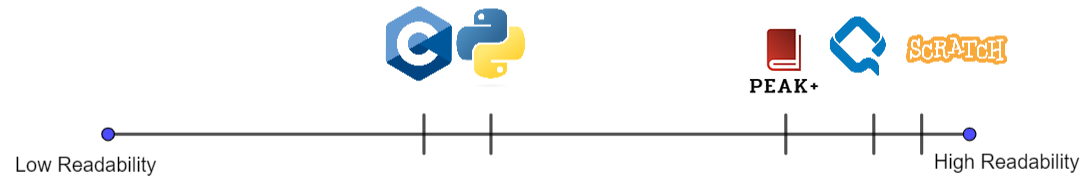
\includegraphics[width=0.9\textwidth]{Files/Billeder: Design/ReadabilityOwn.png}
    \end{center}
    \caption{The programming languages C, Python, Quorum, and Scratch placed on a scale showing readability, including \lang.}
    \label{LD:readability_scale}
\end{figure}


\subsection{Writability}
The writability of \lang is lower since the language should relate to concepts and terminology from high school education. Therefore the language syntax should resemble the English language and math learned in high school. The purpose of \lang is to enable an easy learning curve of the fundamental concepts and implementations used by many of the common industry programming languages.  Furthermore, as \lang is intended to be an introductory language, a focus of the language will not be creating large and optimized applications. \\

That being said, one goal of \lang is to introduce beginner programmers to the use of methods and procedures, which supports a level of abstraction within the language. Because methods are a core principle within programming, they will be implemented, in a manner that supports readability.\\

On the scale displayed in figure \ref{LD:Writability_Scale}, \lang has been placed between C and Quorum, but closer to C. This is due to the fact that the language will have low expressivity, limited support for abstraction (no object-oriented constructs), and a limited amount of data types. Like Quorum, the focus of this language is more on readability in preference to writability. Like Quorum, the goal will be for beginners to be able to quickly recognize and understand the language, and therefore most reserved keywords will not be abbreviations like in many languages.


\begin{figure}[H] 
    \begin{center}
        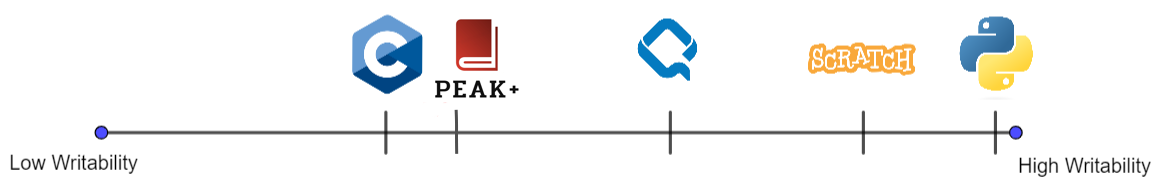
\includegraphics[width=0.9\textwidth]{Files/Billeder: Design/WritabilityOwn.png}
    \end{center}
    \caption{The programming languages C, Python, Quorum, and Scratch placed on a scale showing writability, including \lang.}
    \label{LD:Writability_Scale}
\end{figure}

\subsection{Reliability} \label{LanguageDesign:Realiability}
The importance of reliability is to ensure that the language does what the programmer specifies it to do, within the boundaries of the language. In \lang, there are certain standards that need to be upheld within reliability, in order to cater to a beginner programmer. \\

The language will use static type checking, which should increase the reliability compared to dynamic type checking since the programmer will have to make sure types are appropriately used. On top of this to further simplify the language and improve reliability, aliasing will be restricted by not allowing pointers in the language. From our personal experience, pointers are a tricky programming construct to understand and use, and it is therefore inappropriate to allow aliasing in a language made for beginner programmers. As \lang will have limited or restricted aliasing and no exception handling, it is placed between C and Quorum on the reliability scale in figure \ref{LD:reliability_scale}.

\begin{figure}[H] 
    \begin{center}
        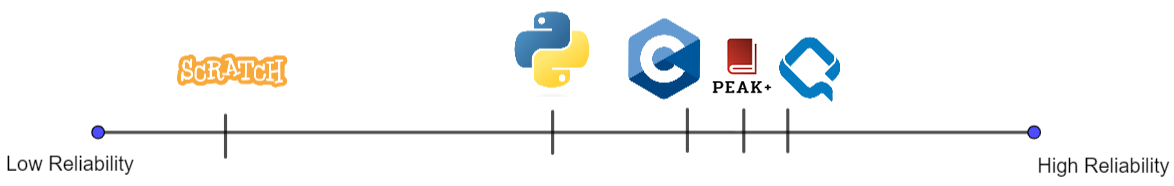
\includegraphics[width=0.9\textwidth]{Files/Billeder: Design/ReliabilityOwn.png}
    \end{center}
    \caption{The programming languages C, Python, Quorum, and Scratch placed on a scale showing reliability, including \lang.}
    \label{LD:reliability_scale}
\end{figure}


\section{The Paradigm of \lang}
Because the goal is to make a beginner-friendly programming language, which aims to make it easier for its users to transition to industry standard languages, the chosen paradigm for \lang is an imperative and procedural paradigm. They have been chosen because, in our own experience, it is important to learn basic programming concepts first like defining basic programming instructions and scopes. An object-oriented approach is deemed too advanced and unnecessary, as we only want to include basic concepts such as functions, control structures, and some basic data types. The same reasons apply to why the functional paradigm has not been chosen. The paradigms mentioned here have been previously explained in section \ref{text-basedlanguages}

\section{Requirements} \label{requirements}
In order to develop a programming language for beginner programmers, requirements must be set. The requirements for \lang are displayed in table \ref{tab:requirements}. 

\begin{table}[H]
\resizebox{\textwidth}{!}{%
\begin{tabular}{|l|ll}
\hline
\textbf{Priority} & \multicolumn{1}{l|}{\textbf{ID}} & \multicolumn{1}{l|}{\textbf{Requirements}} \\ \hline
\multirow{6}{*}{Must Have} & \multicolumn{1}{l|}{M1} & \multicolumn{1}{l|}{\begin{tabular}[c]{@{}l@{}}Declaration and assignment of number, decimal, text, \\ and boolean variables.\end{tabular}} \\ \cline{2-3} 
 & \multicolumn{1}{l|}{M2} & \multicolumn{1}{l|}{Display output and take keyboard input in the console.} \\ \cline{2-3} 
 & \multicolumn{1}{l|}{M3} & \multicolumn{1}{l|}{Basic iterative and selective control structures} \\ \cline{2-3} 
 & \multicolumn{1}{l|}{M4} & \multicolumn{1}{l|}{Basic arithmetic \& logical operations.} \\ \cline{2-3} 
 & \multicolumn{1}{l|}{M5} & \multicolumn{1}{l|}{\begin{tabular}[c]{@{}l@{}}Syntax which resembles concepts and terminology used in \\ high school education.\end{tabular}} \\ \cline{2-3} 
 & \multicolumn{1}{l|}{M6} & \multicolumn{1}{l|}{Error messages at compile time.} \\ \hline
\multirow{4}{*}{Should Have} & \multicolumn{1}{l|}{S1} & \multicolumn{1}{l|}{A foreach loop.} \\ \cline{2-3} 
 & \multicolumn{1}{l|}{S2} & \multicolumn{1}{l|}{String concatenation.} \\ \cline{2-3} 
 & \multicolumn{1}{l|}{S3} & \multicolumn{1}{l|}{Declaration and assignment of lists.} \\ \cline{2-3} 
 & \multicolumn{1}{l|}{S4} & \multicolumn{1}{l|}{List helper functions like add and remove from the list.} \\ \hline
Could Have & \multicolumn{1}{l|}{C1} & \multicolumn{1}{l|}{Support for abstraction in the form of methods} \\ \hline
Won't Have & \multicolumn{1}{l|}{W1} & \multicolumn{1}{l|}{Exception Handling} \\ \hline
\end{tabular}%
}
\caption{MoSCoW requirement table.}
\label{tab:requirements}
\end{table}


The requirements are designed in the light of the target group, beginner programmers. By looking at several different programming tasks given in different beginner programming courses, more features necessary for a beginner language have been settled, leading to the requirements for \lang. The tasks that are examined, are from the imperative programming course in the first semester of our own education\cite{C-CourseExercises}, Python practice exercises from python.org\cite{PythonBasicsExercise} and general code challenges from codecademy.com \cite{CodeAcademyExercises}. Besides examining programming tasks, the requirements are also defined with the language criteria in section \ref{languageCriteriaForLang} in mind.\\

The language has to implement fundamentals for a programming language, including declarations and assignments of variables (M1) and the ability to generate an output to the console and read keyboard inputs (M2). Another fundamental requirement is the use of different types of control structures, both selective and iterative. Examples of beginner tasks include repeating some code $x$ times or as long as a condition is satisfied. In relation to the decision stated in section \ref{Lang Readability} about \lang prioritizing readability, the control structures in \lang have to be concrete and easy for the beginner programmer to understand. In (M3) the definition of basic control structures includes the implementation of if-else condition blocks, a counting loop and a conditional loop. \\ 

To ensure the readability of \lang, the syntax has to resemble concepts and terminology used in high school, e.g. the use of fully spelled words and basic math symbols, leading to requirements M4 and M5. In addition to this, requirement S2 about string concatenation is implemented, as context to compound words. \\

Since \lang is a beginner language, it is important that there are error messages at compile time. This relates to requirement M6.
\\

Different ways of storing related variables are also common in the tasks. For example, saving several variables in a list, deleting an entry in a list, and getting a variable from an entry in the list, leading to requirements S3 and S4. 
\\

Scopes and Functions are also relevant topics. This entails functions which have the possibility of receiving an input and returning an output. This relates to requirement C1. 
\\

\lang will not have exception handling. This feature is deemed as nice to have, but the aforementioned features have been deemed more important due to having a higher impact on the simplicity of \lang.   


\section{Syntax Design} \label{sec:SyntaxDesign}
To create the language specification for \lang, the first step is defining the syntax. Syntax describes the grammar and structure of valid programs in a language. The syntax design is followed up by operational semantics and type rules in section \ref{operational_Semantics}.
This section will cover theoretical sections about context free grammar and Backus-Naur Form, followed up by the context free grammar for \lang.

% Certain precautions should be noted with the decision of having number and decimal. In order to increase simplicity, the first intuition was to only implement one type \textit{number}, encapsulating both integer numbers and decimal numbers. Generalizing all instances of a number into one type would need to be dynamically handled by the compiler. Furthermore, it could lead to less readability in the language control structures, (ref til section), since counting loops should not work with decimals. In order to deal with this issue, all integer numbers will internally be \textit{number} and all decimal numbers have to be \textit{decimal} 


\subsection{Context-Free Grammars} \label{LD: CFG}
A context free grammar (CFG) is a way to formally represent the syntax of a language using symbols and rules. They describe all possible programs that are syntactically correct in the language. A CFG is specified as having a finite set of terminal and non-terminal symbols as well as a start symbol and a finite set of production rules \cite{SPO_Topic_5}. An example of a CFG is displayed in listing \ref{list:CFGExample}.

\begin{lstlisting}[language=scriptkid, label={list:CFGExample},caption=An example of a CFG. The language accepts strings of zero or more A's followed by a 'b' ]
Start -> A B $
A -> A a | epsilon
B -> b
\end{lstlisting}

A terminal symbol is a symbol from the language's alphabet\cite{SPO_Topic_5}. These are always written in lowercase letters. The non-terminal symbols are placeholders for terminal symbols or patterns of terminal symbols. These are written with the first character in uppercase. Non-terminal symbols are derived into other terminals and/or non-terminals until they become exclusively terminal symbols. This is done using production rules \cite{SPO_Topic_5}. Reviewing the CFG in listing \ref{list:CFGExample}, it can consists of several production rules. A production rule describes a possible way, in which a non-terminal can expand. The LHS (left-hand-side) of the arrow in each production rule consists of a non-terminal, that is to be derived. The rules to derive the nonterminal are given by the RHS (right-hand-side). There can be several different ways a non-terminal can be rewritten. The different production rules for a non-terminal are separated by a line '|' and can contain combinations of terminals and non-terminals as well as having the possibility of being epsilon ($\epsilon$), meaning an empty string. Furthermore, the first non-terminal in the LHS of the CFG is the start symbol \cite{SPO_Topic_5}. \\
The terminals in the example in listing \ref{list:CFGExample} are \textit{a}, \textit{b}, and \textit{\$}. The start symbol is 'Start' which can be derived into \textit{A B} followed by the \textit{\$}, end of input stream symbol. The process continues until no non-terminal remains in the derived string. In listing \ref{list:CFGExample}, \textit{A} is either derived to epsilon at the beginning or recursively derived into \textit{A a} until the nonterminal \textit{A} derives into epsilon. Furthermore, \textit{b} is derived from the nonterminal \textit{B}. \\

A CFG can be represented using BNF (Backus-Naur Form) or EBNF (Extended Backus-Naur Form). The set of strings that a CFG can define is called its language. A string that belongs to the language of the CFG, can be considered a valid string for the CFG \cite{SPO_Topic_5}. The notation of a CFG can vary, but in this report, productions for non-terminals are shown using an arrow '->'.

\subsection{Backus-Naur Form}
BNF (Backus-Naur Form) and EBNF (Extended Backus-Naur Form) are two ways to represent a CFG\cite{SPO_Topic_5}. In \lang, BNF has been used to represent the CFG. An advantage of using BNF over EBNF is that BNF is simpler in the way that it only uses a small set of metacharacters\cite{IBM} and rules which are easy to learn and understand. A disadvantage of using BNF instead of EBNF is that BNF uses a larger amount of productions to describe the same grammar as EBNF. This can make the grammar more difficult to read than EBNF which can especially be a problem when creating complex grammar.\\ 
EBNF extends BNF by using elements similar to regular expressions, such as "[]" to indicate an optional element or "\{\}" to indicate repetition zero or more times\cite{SPO_Topic_5}.\\
Overall, the advantages of using BNF are that it is simpler to learn and understand, as it has fewer metacharacters. Furthermore, most CFG tools do not recognize EBNF. For these reasons, we will write the CFG of \lang using BNF.

\subsection{Context-Free Grammar for \lang} \label{CFGForLang}
The \lang programming language focuses on being simple in its syntax and data structures, while also implementing common principles from the programming industry for an easier transition from a beginner language to a language such as C or C\#.\\

In order to make the language easier to understand for new programmers, only 5 data types will be implemented. Three of these data types are primitive, being \textit{number}, \textit{decimal} \& \textit{boolean}. The other two are non-primitive data types being \textit{text} \& \textit{list}. The data type \textit{number} is an integer, and \textit{decimal} is a floating point number. To increase readability, the \textit{boolean} is a boolean value, having either the value \textit{true} or \textit{false}. Conditional operators taught in high school mathematics are included, such as '\textit{<}' and '\textit{<=}'. The logical \textit{or} and the logical \textit{and} are written in text as these operators are not introduced in the high school curriculum. \textit{text} is a string, which is a collection of characters, and \textit{list} is a collection of any of the previous types. \\
% and a feature that is aimed to be implemented is string concatenation via the "+" operator. This allows for better readability of strings. 

%Any instance of the \textit{text} variable will be seen by the compiler as a collection of chars. In regards to string manipulation. Another feature that is aimed to be implemented is string concatenation via the "+" operator. This allows for better readability of strings. \lang will also implement \textit{Lists} as a type, which aims to generalize any collection of a single type into one data type. \\ This highlights simplicity and orthogonality within \lang. 

\textbf{Overall program structure:} The overall structure of the \lang programming language can be seen in listing \ref{list:CFGOverallStructure}. A program in \lang consists of a list of commands, which can be further broken down into either a statement or a declaration. A declaration consists of a type, an id, and an optional assignment, whereas a statement can be broken further into multiple different productions. Like in many other languages, a semicolon ';' is used as a statement terminator, making it clear when a statement ends. Using semicolons as a statement terminator instead of, for example, a newline, also allows the programmer to span a long statement across multiple lines, making it more readable. This makes it so anyone reading the code is able to read a long statement without having to scroll left and right in their editor. It also allows for multiple statements on a single line.\\

\begin{lstlisting}[language=scriptkid, label={list:CFGOverallStructure},caption=Overall structure of \lang CFG]
Program        -> Cmds 
Cmds           -> Cmd Cmds | EPSILON 
Cmd            -> Stmt | Dcl 
Dcl            -> Type Id Ass ; 
Ass            -> = Expr | EPSILON 
Stmt           -> Id = Expr ; | CtrlStrct | ListStmt ; | FuncDef | FuncCall ;
\end{lstlisting}

\noindent\textbf{Control structures: } The control structures of \lang can be seen in listing \ref{list:CFGCtrlStrct}. A control structure in \lang can be either a selective control structure (if statement), or an iterative control structure (loop). This can be seen from the Non-terminal \textit{CtrlStrct} in listing \ref{list:CFGCtrlStrct}, which can derive from the productions \textit{IfStmt} or \textit{Loop}. \\ 
When deciding on control structures, the standard if-else blocks are used to support readability. However, in regards to loops, it has been decided to generalize all loops by using the reserved word \textit{repeat}, instead of the standard \textit{for} and \textit{while}. This is based on the analysis of the Quorum programming language, which simplifies the standard loop structures. 
\\

\begin{lstlisting}[language=scriptkid, label={list:CFGCtrlStrct},caption=Control structure of \lang CFG]
CtrlStrct -> IfStmt | Loop   
IfStmt -> if ( Expr ) Block ElseIfStmt   
ElseIfStmt -> else if ( Expr ) Block ElseIfStmt | Else | EPSILON   
Else -> else Block   
Loop -> repeat Loops   
Loops -> LoopStmt | WhileStmt | ForeachStmt   
LoopStmt -> ( Expr ) times Block 
WhileStmt -> while ( Expr ) Block   
ForeachStmt -> for each ( Type Id in Id ) Block   

\end{lstlisting}

\noindent \textbf{If statement: } An if statement in \lang starts with the terminal keyword \textit{if}, followed by an \textit{Expr} nonterminal encapsulated by parentheses, a \textit{Block} and an optional \textit{ElseIfStmt} (See line 2 in listing \ref{list:CFGCtrlStrct}). An \textit{ElseIfStmt} production has the same structure as an \textit{IfStmt}, but with the terminals \textit{else if} instead of just \textit{if}. Furthermore, it derives to the nonterminal \textit{Else} and \textit{EPSILON}, making the \textit{ElseIfStmt} optional as it has a production that derives to nothing. An advantage of this structure is that it allows for checking multiple expressions and even nesting if statements, which makes writing complex conditional logic easier. However, this can also turn into a disadvantage, as deeply nested code may confuse the programmer as it will be harder to read and understand.\\

%An advantage of this structure having a \textit{Block} in an if statement, and a block being able to derive back to an if statement, is that it allows for nested conditional statements. Howe\\\

\textbf{Loops: } A loop in \lang will always derive to the \textit{repeat Loops} production as can be seen on line 5 in listing \ref{list:CFGCtrlStrct}. This means that any loop will consist of the terminal keyword \textit{repeat}, followed by one of the different loop types defined in listing \ref{list:CFGCtrlStrct}. Having the structure consist of the terminal \textit{repeat} followed by a loop type, provides a consistent way to define and identify loops in \lang. A disadvantage of this is that it adds an extra word to the language every time a loop is created, which gives the language slightly less writability. However, as previously mentioned in section \ref{Lang Readability}, readability is prioritized above writability in \lang.\\

\lang has three kinds of loops being a counting loop, a while loop, and a for each loop. The counting loop has the following syntax: "repeat (x) times{}". This is a simple loop, which is intended for beginners to get familiar with loops in their simple form. The loop requires an integer number or variable of the type \textit{number} to determine how many times the loop should run. The while loop functions as in any other programming language, where it runs as long as a condition is fulfilled. The while loop is deemed necessary for the language, as it is able to achieve more than other loop constructs. Finally, the \textit{for each} loop has been selected for the \lang language in order to provide a simple way of looping through each element in a collection. This is simpler than a normal \textit{for} loop as a \textit{for each} loop only requires an initializer expression and the collection to loop through. In comparison, a for loop requires both an initializer expression(s), a continue expression, and an update expression(s). A for-loop syntax may be difficult for beginner programmers to remember, so, therefore, a for-loop control structure will not be included in the language. \\

\textbf{Functions: } The function definition of \lang can be seen in listing \ref{list:CFGCtrlStrct}. A function definition in \lang starts with the terminal \textit{function} followed by an \textit{Id}, a list of parameters, the function return type, and finally the function body. 

\begin{lstlisting}[language=scriptkid, label={list:CFGFunction},caption=Function call \& declaration of \lang CFG]
FuncCall -> call Id ( ArgList ) | call output ( ArgList ) | call Type input ( ArgList ) 
FuncDef -> function Id ( ParamList ) FuncReturn Block   
FuncReturn -> return FuncReturnType   
FuncReturnType -> Type | nothing   
ParamList -> Param ParamTail | EPSILON   
ParamTail -> , Param ParamTail | EPSILON   
Param -> Type Id   
ArgList -> Expr ArgTail | EPSILON   
ArgTail -> , Expr ArgTail | EPSILON   

\end{lstlisting}

The \textit{function} terminal is used in order to clearly define that a function is being defined, increasing readability. The return type is placed after the parameter list. This choice is made in order to obtain readability by separating the return type from the start of the declaration. Explicitly having to use the return keyword along with the function keyword in a function definition provides less writability, but more readability. 
The \textit{FuncReturnType} nonterminal derives to either a \textit{Type}, or \textit{nothing}. The \textit{nothing} return type is equivalent to the void return type in other languages. The \textit{nothing} keyword is used instead, due to the fact that returning \textit{nothing} seems more intuitive than \textit{void} for beginner programmers. 

The \textit{FuncCall} nonterminal has one production, starting with the terminal \textit{call}, followed by an \textit{Id} and an \textit{ArgList} enclosed by parentheses. The \textit{call} keyword is used to once again increase readability, as it helps clearly define when a function is called. \\

\textbf{Input \& output: } The definition of input and output for \lang can be seen in listing \ref{list:CFGInputoutput}. The \textit{output} terminal is used as a way to write / print something to the console. Whereas the \textit{input} terminal is a way to read input from the user. 
\begin{lstlisting}[language=scriptkid, label={list:CFGInputoutput},caption=Input \& output of \lang CFG]
FuncCall -> call Id ( ArgList ) | call output ( ArgList ) | call Type input ( ArgList )
.
.
.
ArgList -> Expr ArgTail | EPSILON   
ArgTail -> , Expr ArgTail | EPSILON 
\end{lstlisting}
The input and output definition starts with the non-terminal \textit{FuncCall} which can derive to either \textit{call output} or the \textit{call Type input}. As can be seen in listing \ref{list:CFGInputoutput}, both the terminal \textit{input} and the terminal \textit{output} takes the non-terminal \textit{ArgList} as a parameter. The non-terminal \textit{ArgList} derives into an expression followed by the next non-terminal \textit{ArgTail}. In the CFG, the input may contain multiple expressions. However, in the compiler, the \textit{ArgList} for the input function should only be able to contain a single expression, being a variable of the type defined after the \textit{call} terminal. The reason for using \textit{ArgTail} instead of \textit{Id} in the input even though the input is essentially an id, is to keep consistency among functions, following the general function definition structure. 
\\

\textbf{Lists:} A list in \lang starts from the non-terminal \textit{Stmt} which then derives to the non-terminal \textit{ListStmt} production as can be seen in listing \ref{list:CFGList}.
\begin{lstlisting}[language=scriptkid, label={list:CFGList},caption=Lists in \lang CFG]
Program -> Cmds   
Cmds -> Cmd Cmds | EPSILON   
Dcl   
Dcl -> Type Id Ass ;   
Ass -> = Expr | EPSILON   
Stmt -> Id = Expr ; | CtrlStrct | ListStmt ; | FuncDef | FuncCall ; | CommentStmt ; | return Type ; 
.
.
.
ListStmt -> ListOpr | ListOprExpr 
ListOpr -> Id : Add ( ArgList ) | Id : Replace ( ArgList ) 
ListOprExpr -> Id : IndexOf ( Expr ) | Id : ValueOf ( ArgList ) 
\end{lstlisting}
The non-terminal \textit{ListStmt} can derive either the non-terminal \textit{ListOpr} or the non-terminal \textit{ListOprExpr}. A \textit{ListStmt} will always start with the terminal \textit{Id}, which refers to the Id of the list being operated on. If going from the non-terminal \textit{ListOpr} it is possible to derive to the terminal \textit{Add}, to add an element to the list, or derive to the terminal \textit{Replace} in order to replace an element in the list.\\
The non-terminal \textit{ListStmt} can also derive from the non-terminal \textit{ListOprExpr}. The \textit{ListOprExpr} can derive into the terminal \textit{IndexOf} to get the index of a position in the list, or the terminal \textit{ValueOf} to get the value stored in a specific position in the list.


\subsection{Operator Precedence} \label{OrderPrec}
Operator precedence defines the order in which operators are evaluated in an expression. The operator precedence for \lang follows the basic mathematics rules, this can be seen in table \ref{tab:OperatorPrecedence}. The highest precedence in \lang follows the mathematical PEMDAS operators which are: parenthesis, exponent, multiplication, division, addition \& subtraction\cite{mathnasium}. The exponent operator is not included in the language, as it is achievable through multiplication, and therefore is not strictly necessary. Following the PEMDAS operators come the relational operators, such as "\textit{greater than}" and Logical operators such as "\textit{and}". These have the lowest precedence in \lang. This is because the logical operators are typically used in conjunction with operators with higher precedence to combine or negate a result.


\begin{table}[H]
\centering
\begin{tabular}{|l|l|l|}
\hline
\multicolumn{1}{|c|}{Precedence} & Operator & Description \\ \hline
1 & (  ) & Parenthesis \\ \hline
2 & \begin{tabular}[c]{@{}l@{}}x * y\\ x / y\end{tabular} & \begin{tabular}[c]{@{}l@{}}Multiplication\\ Division\end{tabular} \\ \hline
3 & \begin{tabular}[c]{@{}l@{}}x + y\\ x - y\end{tabular} & \begin{tabular}[c]{@{}l@{}}Addition\\ Subtraction\end{tabular} \\ \hline
4 & \begin{tabular}[c]{@{}l@{}}x \textgreater  y\\ x \textgreater{}= y\\ x \textless y\\ x \textless{}= y\end{tabular} & \begin{tabular}[c]{@{}l@{}}Greater than\\ Greater than or equal to\\ Less than\\ Less than or equal to\end{tabular} \\ \hline
5 & \begin{tabular}[c]{@{}l@{}}x is y\\ x is not y\end{tabular} & \begin{tabular}[c]{@{}l@{}}Is equal to\\ Is not equal to\end{tabular} \\ \hline
6 & x and y & Logical and operator \\ \hline
7 & x or y & Logical or operator \\ \hline
\end{tabular}
\caption{Operator Precedence for \lang}
\label{tab:OperatorPrecedence}
\end{table}

\subsection{Scope Rules} \label{sec:scope_rules}
Scope rules regulate the visibility of identifiers in a programming language. They relate every applied occurrence of an identifier to a binding occurrence. The binding occurrence is defined as the instance where an identifier is declared initially, and the applied occurrence is any point at which the identifier is used as part of an expression \cite{craftingcompiler}. Both of these occurrences can be seen in listing \ref{list:binding}. Different scope rules give rise to different interpretations of the same piece of code \cite{transtrees}. 

\begin{lstlisting}[language = scriptkid, label={list:binding},caption=Example of a binding occurence and an applied occurence of the identifier \textit{x} in \lang]
number x = 1; // Binding Occurence

number r = x + 1; // Applied Occurence
\end{lstlisting}

\noindent
There are two kinds of scope rules: Dynamic and static. Dynamic scope rules employ the bindings known when the procedure is called and are based on the program's runtime. Static scope rules employ the bindings known when the procedure is declared and are based on the structure of the program\cite{transtrees}. \lang will use static scope rules. The main reason for this choice is to strengthen the readability of \lang. \lang uses the nested block structure. A nested block structure means, that a program can be subdivided into several disjoint blocks with an infinite amount of blocks inside each block. A block is an area of text in the program that corresponds to some kind of boundary for the visibility of identifiers. The essence is that several local definitions of a single identifier may occur in different blocks (but not in the same block) \cite{craftingcompiler}.
The reason for this is to enable flexibility for the beginner programmer. A nested block structure is also a common industry standard, which prepares the programmer for those languages. The scope rules for \lang are:

\begin{itemize}
  \item A \textit{block} in \lang can be a \textit{function} or control structure, like \textit{if}-statements. \lang also contains special characters like \textit{repeat} and \textit{repeat for each} that iterate over a block a defined amount of times.
  \item All blocks are defined by using the prefix for one of the above and encapsulating the content between two curly brackets, this can be seen in listing \ref{list:block}.
  \item A local variable declared inside a block can only be applied within that block and any nested blocks within it. Variables declared globally can be used anywhere.
  \item Variable shadowing is allowed within nested blocks.
  \item  
  Functions have to be declared in the global scope, and cannot be redeclared in any scope. 
\end{itemize}

\begin{lstlisting}[language=scriptkid, label={list:block},caption=Example of a Block]
function Sum(number x, number y) return number 
{ 
    return = x + y; 
} 
\end{lstlisting}

\newpage
\section{Semantics}
To settle the behavior of the language, the next step in the language specification for \lang is defining the semantics. This section covers abstract syntax, type rules, and operational semantics. The subsections will be structured with theoretical knowledge, followed up by the constructs from \lang. \\

The source of the knowledge described in this section is from the course Syntax and Semantics and will be cited in the paragraph when appropriate. Definitions that are directly from the course material, will also have standard citations, without quotation marks.

\subsection{Abstract Syntax} \label{AST}
%Within most compilers, there exists a phase in which the parse tree derived from the program, is transformed into an abstract syntax tree (AST). The AST simplifies the program, making it easier to handle when further decorating the tree and eventually in the code generation phase. This is further explained in \ref{ASTDesign}.\\

Abstract syntax defines the structure of valid programs in the language but in a more abstract and simplified form. It is for example not concerned with parsing and ambiguity problems and it does not have to comply with the standard formats for parsing algorithms\cite{SS_lecture_8}. The abstract syntax is defined from a combination of a set of syntactic categories, which are seen in table \ref{tab:SyntacticCategories}. A set of formation rules is defined for these syntactic categories, which can be seen in table \ref{tab:formationrules} \cite{SS_lecture_8}. \\

\begin{table}[H]
\begin{tabular}{llll}
\textit{n}   & 	\in & \textbf{Num}     & Natural Numbers       \\
\textit{d}   & \in  & \textbf{Dec}     & Rational Numbers      \\
\textit{txt} & 	\in & \textbf{Text}    & Strings               \\
$\mathbb{T, F}$  & \in & \textbf{Bool}   & Boolean values        \\
\textit{x}   & 	\in & \textbf{Var}     & Variable names        \\
\textit{L}   &  \in & \textbf{List}    & Lists                  \\
\textit{f}   & 	\in & \textbf{Func}    & Function names        \\
\textit{B}   & 	\in & \textbf{BTypes}  & Base Types            \\
\textit{T}   & \in & \textbf{Types}      & All Types             \\
\textit{e}   & 	\in & \textbf{Exp}     & Expressions           \\
\textit{S}   & 	\in & \textbf{Stm}     & Statements            \\
$D_V$           & \in & \textbf{DecVar}  & Variable declarations \\
$D_F$           & \in & \textbf{DecFunc} & Function declarations
\end{tabular}
\caption{Syntactic categories of \lang}
\label{tab:SyntacticCategories}
\end{table}

\noindent The syntactic categories in table \ref{tab:SyntacticCategories} represent all elements in \lang. To represent an element of the syntactic categories we use meta-variables, which are the characters in the first column in the table. E.g the syntactic category \textbf{Num} in the first row, represents any natural number in \lang and the meta variable \textit{n} is used in the abstract syntax to represent an arbitrary number. Lists are defined using $L$ and contain any amount of expressions in an ordered format.\\ 

%Besides numbers, the goal is to implement a decimal value as well, in order to handle certain divsions and general arithmetic's with decimal numbers. The problem with generalizing every \textbf{Num} instance into a floating point number, is that non-integer numbers are generally not compatible with indexing lists.The \textbf{Text} variables are handled as a sequence of characters. \textbf{Lists} are stored in the heap, in order to dynamically declare them, the reason for this is to increase flexibility of the language, in order to cater towards beginner programmers. 

\begin{table}[H]
\resizebox{\columnwidth}{!}{%
\begin{tabular}{lll}
\textit{B}  & ::= & number | decimal | text | boolean  \\ \\
\textit{T}  & ::= & \textit{B} | list(\textit{B}) \\ \\
\textit{e}  & ::= &
  \begin{tabular}[c]{@{}l@{}} 
  $n$ | $txt$ | $\mathbb{T}$ | $\mathbb{F}$ | $d$ | $x$ | $e_1$ + $e_2$ | $e_1$ - $e_2$ | $e_1$ * $e_2$ | $e_1$ / $e_2$ | $e_1$ is $e_2$ | $e_1$ is not $e_2$ |\\ $e_1$ > $e_2$ | $e_1$ >= $e_2$ | $e_1$ < $e_2$ | $e_1$ <= $e_2$ | $e_1$ and $e_2$ | $e_1$ or $e_2$ | ($e_1$) | $x$:valueOf($n$) | $x$:indexOf($e$)
  \end{tabular} \\ \\
\textit{S} &
  ::= &
  \begin{tabular}[c]{@{}l@{}} $S_1$ ; $S_2$ | $D_V$ | $D_F$ | $x$ = $e$ | $x$:add($e_1$ , ... , $e_k$) | $x$:insert($e$ , $n$) | \\ if($e$) \{ $S$ \} | If($e$) \{ $S_1$ \} Else \{ $S_2$ \} | repeat ($n$) times \{ $S$ \} | repeat while ($e$) \{ $S$ \} | \\ repeat for each ($B$ $x$ in $x$) | call $f$($e_1$, ... , $e_k$) | x = call $f$($e_1$, ... , $e_k$) | $\epsilon$\end{tabular}\\ \\
$D_V$ & ::= & $T x = e$ ; $S$ | $T x$ ; S | $\epsilon$                   \\ \\
$D_F$ & ::= & function $f$($T_1\ x_1$ , ... , $T_k\ x_k$) return $T$ \{ S_1 ; \ $return$ \ e \} ; \ S_2\ |\ $\epsilon$ \\ \\
\end{tabular}%
}
\caption{Abstract Syntax formation rules}
\label{tab:formationrules}
\end{table}

\noindent The formation rules define the structure of the syntactic categories and are written in the same format as production rules in BNF, explained in section \ref{LD: CFG} \cite{SS_lecture_8}. In the first column in table \ref{tab:formationrules}, it is denoted that an expression \textit{e} in \lang can be one of the related right-hand side formation rules. \\

The syntactic categories \textbf{Num}, \textbf{Dec}, \textbf{Text}, \textbf{Bool}, \textbf{Var} and \textbf{Func} do not have formation rules as they are trivial. For example, \textbf{Text} is a string of characters, as explained in section \ref{LD: CFG}. 

\subsection{Type Rules} \label{sec:TypeRules}
To prevent a program to execute with errors, a type system is important. When compiling a program, the type systems' purpose is to catch type errors before the program executes. When a program executes without type errors it is called \textit{well-typed}. To know when a program is well-typed, we define type rules. The type rules of a language define how the different types in the language are allowed to be used correctly. \\

%Henceforth, type checking will be done at compile time. Additionally, \lang will use dynamic binding, meaning all variable declarations can be reassigned, and re-declared within a nested scope. Functions can be declared once within a specific scope. 

In the type system, values of variables are kept in an environment. As variables get declared or reassigned, they are updated in the environment \cite{SS_lecture_10}. A type environment keeps track of the types of variables. A type environment is a partial function that maps variables to types, \textit{E} : \textbf{Var} $\cup$ \textbf{Func} $\rightharpoonup$ \textbf{Types} \cite{SS_lecture_10}. When the state is changed in the environment it can be denoted as $E[x \mapsto T]$. The formal definition of an update to the environment is the following function:

\begin{equation}
    (E[x\mapsto T])(y) = \begin{cases}E(y) &  y \neq x\\T & y = x\end{cases}
\end{equation}

\noindent To define a type system, the first step is to describe a collection of formal statements called \textit{judgments} \cite{SS_lecture_10}. The two types of judgments that are used in the type system, are seen in definition \ref{judgments}\cite{SS_lecture_10}. 
\begin{equation} \label{judgments}
    \begin{split}
        E \vdash e:T \\ E \vdash S:ok
    \end{split}
\end{equation}

\noindent
In definition \ref{judgments} it can be read as, within the environment \textit{E} some assertion of a syntactic category is made. In the first judgment, we assert that an expression \textit{e} has a certain type, and in the second judgment, we assert that a statement \textit{S} is well-formed in accordance with the formation rules. The judgment will be derived from the type rules defined in the type system. Such derivations can be used to describe this system. Definition \ref{derivation_example} is the template for how the derivations will be presented\cite{SS_lecture_10}.

\begin{equation} \label{derivation_example}
    \frac{E_1 \vdash \alpha_1 , ..., E_n \vdash \alpha_n}{E \vdash \alpha}
\end{equation} 

\noindent The $\alpha$ represents a syntactic category implementation and can be any of the two mentioned judgments in definition \ref{judgments}. Based on the explained rules, the type system of \lang can be formally described. \\

The standard derivation for a variable can be performed when a variable reaches its final possible derivation. In definition \ref{Varts} the derivation checks if a variable's type matches what is in the environment.

\begin{equation} \label{Varts}
    (VAR_{TS})\frac{E(x) \ = \ T}{E \ \vdash x \ : \ T}
\end{equation} \\

\noindent As mentioned in section \ref{sec:scope_rules}, \lang allows 
variable shadowing, meaning a variable can be redeclared in an inner scope. Furthermore, type errors can occur when expressions are made with types that are not compatible. 
Firstly, the type rules for expressions can be seen in definitions \ref{expression_rules}, \ref{Dec*_ts}, \ref{TXTts}, and \ref{Bool*_ts}.

\begin{equation} \label{expression_rules}
  (NUM*_{TS})\frac{E \ \vdash \ e_1 : \ number \ E \ \vdash \ e_2 : \ number \ }{E \ \vdash e_1 \star \ e_2 \ : \ number} \ \ \ \
  where \ \star \in \{ +, *, - \}  
\end{equation}
    
\begin{equation} \label{Dec*_ts}
    (DEC*_{TS})\frac{E \ \vdash \ e_1 : \ decimal \ E \ \vdash \ e_2 : \ decimal \ }{E \ \vdash e_1 \star \ e_2 \ : \ decimal} \ \ \ \
    where \ \star \in \{ +, *, - , /\},\ and\ e_2 \neq 0
\end{equation}
    
\begin{equation} \label{TXTts}
        (TXT_{TS})\frac{E \ \vdash \ e_1 : \ text \ E \ \vdash \ e_2 : \ text \ }{E \ \vdash e_1 + \ e_2 \ : \ text} 
\end{equation}

\begin{equation} \label{Bool*_ts}
    (BOOL*_{TS})\frac{E \ \vdash \ e_1 : \ number \ E \ \vdash \ e_2 : \ number \ }{E \ \vdash e_1 \star \ e_2 \ : \ boolean} \ \ \ \
    where \ \star \in \{ >, <, \geq, \leq, is, is \ not \}
\end{equation}

\noindent Addition can occur both in an arithmetic sense between \textbf{Num} and \textbf{Dec}, and in the form of string concatenation. However, string concatenation can only occur between two \textbf{Text} variables.  \textbf{Num} \& \textbf{Dec} is mainly split up to avoid conflicts when using a floating-point value as a list index. In definition \ref{expression_rules} the star cannot be a division symbol. If two numbers are divided, the type will convert to a decimal. It is also not allowed to divide by zero. The rest of the type rules for expressions in \lang are found in appendix \ref{Appendix:TypeSystem} \\

The next syntactic category to define type rules for is variable declarations (meta variable $D_V$ in table \ref{tab:formationrules}). These formation rules allow the declaration and assignment of variables with type \textbf{T}. The derivations in definitions \ref{TYPERULE:Dcl} and \ref{TYPERULE:Ass}, describe the type rules. In $(DEC_{TS})$ the $x \ \notin \ dom(E)$ defines that the variable $x$ is not previously in the domain of the environment $E$. This is necessary because a variable declaration creates an instance of a new variable, and there cannot be any existing variables with the same name in the same scope. 

\begin{equation} \label{TYPERULE:Dcl}
    (DEC_{TS})\frac{x \ \notin dom(E) \ \ E \ \vdash \ e : \ T }{E \ \vdash T \ x \ = \ e  \ : \ ok}
\end{equation}

\begin{equation}\label{TYPERULE:Ass}
    (ASS_{TS})\frac{E(x) = T \ \ E \ \vdash \ e : \ T \ }{E \ \vdash x \ = \ e \ : \ ok}
\end{equation}

\noindent The formation rule of $\epsilon$ is shown in definition \ref{epsilonTS}, since it can appear in multiple formation rules. $\epsilon$ simply derives to a well-formed derivation.

\begin{equation} \label{epsilonTS}
    (EMPTYSTM_{TS})\frac{}{\ E \ \vdash \epsilon \ : \ ok}
\end{equation}

\noindent
The last syntactic category which will be shown here is the function declaration. In definition \ref{funcDec1_TS} the function has a return type T. A function declaration is well-formed when the functions block and return value is well-formed in the environment where the variables $x_1,..,x_k$ have the type $T_1,..T_k$. Furthermore, the statement $S_2$ which is executed after the function call is well-formed in the updated environment. \\

Definition \ref{funcDec2_TS} is almost identical to definition \ref{funcDec1_TS}. The change here is, that for a function without a return type, we do not handle the return type in the premises. \\

\begin{equation} \label{funcDec1_TS}
% Type rules for function declaration
(FUNCDEC1_{TS})\frac{\begin{array}{c}
\\ E' \ \vdash \ S_1 : \ ok \ \ \ E' \ \vdash \ e\ : \ T \ \\
E[f \ \mapsto \ 
(x_1 \ : \ T_1 \ , ... , \ x_k \ : 
\ T_k \  \rightarrow \ T)] \ \vdash S_2 \ : \ ok\end{array}  }
{E \ \vdash function \ f(T_1\ x_1 , ... , T_k\ x_k) 
\ return \ T \ \{ \ S_1; \ return \ e \ \}\ ; \ S_2 \ : \ ok}
\end{equation}
\begin{center}
    $where\ E' =\ E[x_1 \ : \ T_1 \ , ... , \ x_k \ : 
\ T_k ]$ 
\end{center}

\begin{equation} \label{funcDec2_TS}
 % Type rules for function call
(FUNCDEC2_{TS})\frac{\begin{array}{c} E[x_1 \ : \ T_1 \ , ... , \ x_k \ : \ T_k \ ] \ \vdash \ S_1 : \ ok \ \\
E[f \ \mapsto \ 
(x_1 \ : \ T_1 \ , ... , \ x_k \ : 
\ T_k \ )] \ \vdash S_2 \ : \ ok\end{array}  }
{E \ \vdash function \ f(T_1\ x_1 , ... , T_k\ x_k) 
\ return \ nothing \ \{ S_1 ; \ return \}\ ;\ S_2 \ : \ ok}
\end{equation}

\noindent There are two ways to handle a function call. As displayed in the formation rules in table \ref{tab:formationrules}, it can either be $call \ f()$ or $x = call \ f()$. In definition \ref{funcCall1_TS}, the left-most derivation checks if there exists a function with the name $f$ which associates to the formal parameters and return type listed. Thereafter each argument given is crosschecked with the appropriate type to make sure they match. If so the derivation is successful. In definition \ref{funcCall2_TS} one more premise is added to the derivation, where we check that the variable $x$ in the environment has type $T$. The rest of the type system can be found in Appendix \ref{Appendix:TypeSystem}.

\begin{equation} \label{funcCall1_TS}
      (FUNCCALL1_{TS})\frac{E(f)\ =\ (x_1: T_1 ,...x_k\ :\ T_k\ \rightarrow\ T) \ \ E \ \vdash \ e_i \ : \ T_i \ }
{E \ \vdash call \ f(e_1,...,e_k) \ : \ ok} \ \ where \ i = 1...k
\end{equation}

\begin{equation}\label{funcCall2_TS}
     (FUNCCALL2_{TS})\frac{E(f)\ =\ (x_1: T_1 ,..., x_k : T_k\ \rightarrow\ T) \ \ E(x)\ = \  T \ \ \ E \ \vdash \ e_i \ : \ T_i \\ }{E \ \vdash x \ = \ call\ f(e_1,...,e_k) \ : \ ok} \ \ where \ i = 1...k
\end{equation}

\subsection{Operational Semantics} \label{operational_Semantics}
Before, the structural operational semantics for \lang can be defined, there is some theory that needs to be explained. Firstly, several forms of semantics exist. Semantics that this report will not cover includes denotational semantics, which focuses on the effect of executing programs by assigning a denotation to them, and axiomatic semantics, which focus on the correctness property of programs \cite{SS_lecture_8}. The semantics that are important to look at in this context are operational semantics. Operational semantics are descriptions of the meaning of a program, precisely telling you how it should execute. To define the operational semantics, we use Transition Systems.

\subsubsection{Transition Systems}
A Transition System is a directed graph and can be defined as a 3-tuple. The formal definition can be seen in definition \ref{transitionSystemTuple} \cite{SS_lecture_8}. 

\begin{equation} \label{transitionSystemTuple}
    S = (\Gamma, \rightarrow, T)
\end{equation}

\noindent The first symbol ($\Gamma$) represents the set of configurations. Each configuration is a vertex of the graph and they represent the current state of the program. An example of this is to think of each vertex containing the known variables which have been declared at that point throughout execution. The arrow symbol ($\rightarrow$) is the transition relation, formally written $\rightarrow \subseteq (\Gamma \backslash T) \times \Gamma$.
%which can be read as a subset of the cross-product between all configurations not including the terminal configurations, to all configurations 
Transitions are the edges of the graph, which act as a bridge between the configurations. From each configuration, you can take the possible transitions to get to another configuration. Each transition is written as a pair ($a$, $b$) where $a$ can transition to $b$. The last symbol ($T$) is the set of terminal configurations. A terminal configuration is a configuration that you cannot transition away from and it is a subset of $\Gamma$, written $T \subseteq \Gamma$. \cite{SS_lecture_8} \\

We took a structural approach to the operational semantics a.k.a (SOS) because it allows us to define the operational semantics based on a few rules. Having SOS means that the transition system has to comply with the following three rules.

\begin{itemize}
    \item Determine the format of the transition (all transitions must comply with the chosen format)\cite{SS_lecture_8}. 
    \item The configurations that are the source of a transition should be terms generated from the abstract syntax in table \ref{tab:formationrules} \cite{SS_lecture_8}.
    \item Define the transition relation by means of structural                 derivation rules\cite{SS_lecture_8}.
\end{itemize} \\

\noindent The format for each syntactical group will be defined later in subsection \ref{TSytstem:Lang} where the transition system for \lang is explained.

%Now that the general concept of the transition system is defined, we can use it to set some \textit{derivation rules} which are "rules that define how the program state changes based on the language construct in focus" \cite{STEP}. The derivation rules will be explained in the following sections using the Big-Step Semantics. 


\subsubsection{Big-Step and Small-Step Semantics} \label{big-step_Chapter}
When deciding to define the operational semantics for a language, two methods can be used. \textbf{Big-Step} semantics and \textbf{Small-Step} semantics. Both of these semantic types can be expressed as the transition system defined in definition \ref{transitionSystemTuple}.

\begin{itemize}
    \item \textbf{Big-Step} semantics (BS) express an entire computation of a given configuration's transition ($\gamma \in \Gamma$) to its terminal configuration ($t \in T$) \cite{SS_lecture_8}. 
    \item "\textbf{Small-Step} semantics (SS) express each transition as a
    single step of a larger computation. Terminal configurations
    characterize when the computation stops" \cite{SS_lecture_8}.
\end{itemize}

\noindent
Small-step semantics are often used when more detail about a derivation is required to understand what is happening. Often it is used in concurrency, where multiple executions in a program are happening at the same time\cite{SS_lecture_12}. For the sake of simplicity as well as the fact that \lang does not have concurrency capabilities, the semantics will be described using Big-Step semantics. \\

To show the basic concept of Big-step semantics, an example of the arithmetic summation of two numbers is shown in definition \ref{bigStep-example}. Here the format of the transition is $a \ \rightarrow _{\textbf{Exp}} v$ where $a \in \textbf{Exp}$ and $v \in \mathbb{Z}$. The transition symbol $\rightarrow _{\textbf{Exp}}$ can be read as "evaluates to an instance of the expression category" \cite{SS_lecture_8}.

\begin{equation} \label{bigStep-example}
    (PLUS_{BS})\frac{a_1 \ \rightarrow _{\textbf{Exp}} \ v_1 \ \ a_2 \ \rightarrow _{\textbf{Exp}} \ v_2}
    {a_1  +  a_2 \rightarrow _{\textbf{Exp}} \ v_1  +  v_2}
\end{equation}

\subsubsection{Environment-Store Model}
Choosing to write the semantics of a programming language in the format shown in definition \ref{bigStep-example} is not extensive enough for \lang. It is unable to handle the scope rules set out for \lang in section \ref{sec:scope_rules} since it assumes a monolithic-block structure. To handle this we use a concept known as the \textit{Environment-Store Model}. This model acts as an addition to the semantics, where it describes how variables are actually bound during execution. Each variable is bound to the location of a storage cell, which holds the value of the variable as its content \cite{SS_lecture_12}.

\begin{figure}[H]
    \centering
    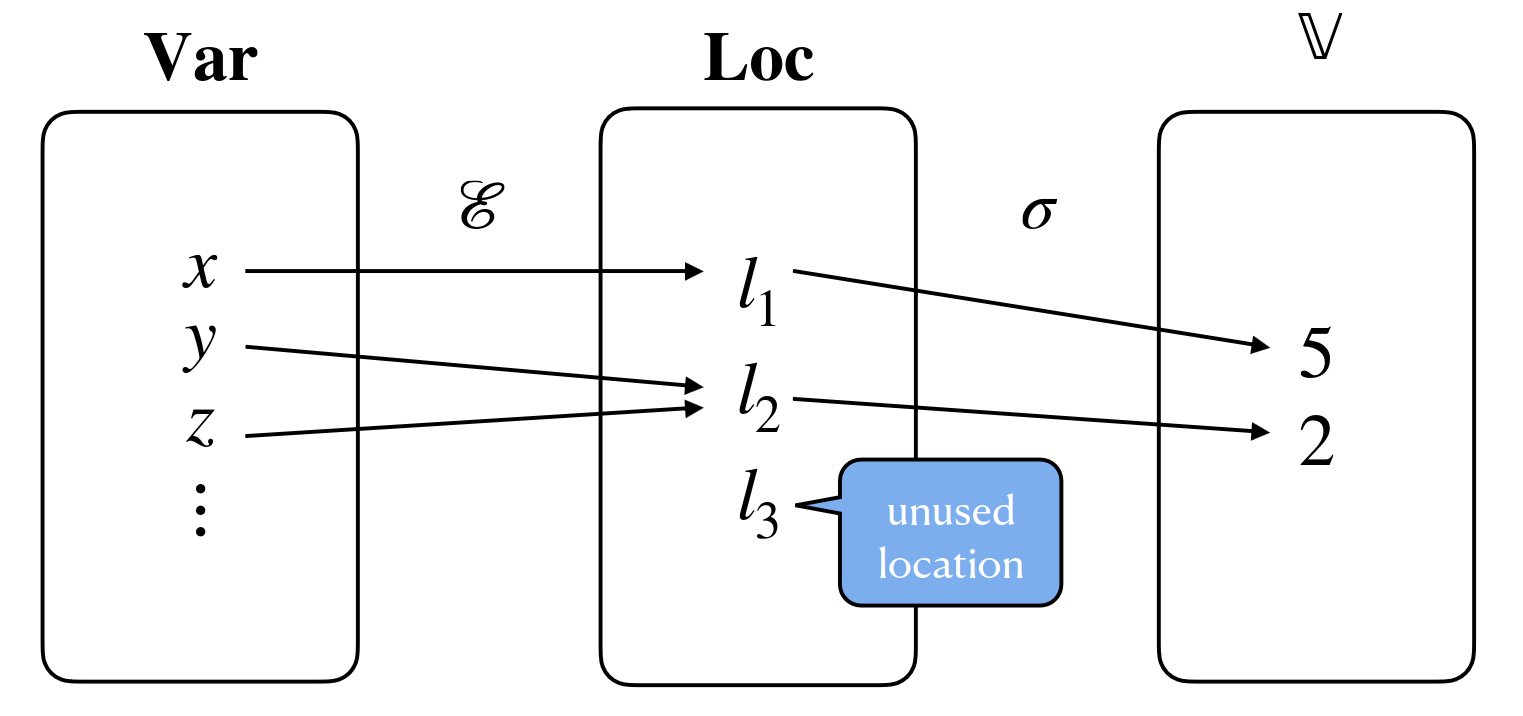
\includegraphics[width=\textwidth]{Files/Billeder: Design/ENVMODEL.png}
    \caption{Visualization of Environment-Store Model \cite{SS_lecture_12}}
    \label{fig:EnvModel}
\end{figure}

\noindent In order to understand the semantics that is defined using the environment-store model, we need to have three definitions in place.

\begin{itemize}
    \item \textbf{Variable Environment:} A partial function that tells which storage location each variable is bound to \cite{SS_lecture_12}. The set of variable environments will be defined as the following:
    \begin{table}[H]
    \centering
    \begin{tabular}{l|l}
    \textit{Single Instance} & \textit{Set of Variable Environments} \\
    $Env_v : \textbf{Var} \rightharpoonup \textbf{Loc}$       & $\mathbf{Env_V} = \textbf{Var} \rightharpoonup \textbf{Loc}$                          
    \end{tabular}
    \end{table}

    \item \textbf{Function Environment:} Describes the content of function name bindings. Essentially the name of a function is bound to the statements and parameters inside of its block, as well as the variable environment given at that time, in order to keep the variable environment statically bound. The function environment will be denoted as the following:
    \begin{table}[H]
    \centering
    \begin{tabular}{l|l}
    \textit{Single Instance} & \textit{Set of Function Environments} \\
    $Env_f : \textbf{Func} \rightharpoonup \textbf{Stm} \ \times \ \textbf{Var} \ \times \ \mathbf{Env_V}$       & $\mathbf{Env_F} = (\textbf{Func} \rightharpoonup \textbf{Stm} \ \times \ \textbf{Var} \ \times \ \mathbf{Env_V})^*$                         
    \end{tabular}
    \end{table}
        
    \item \textbf{Store:} A partial function which describes the content of a storage cell corresponding to a given location \cite{SS_lecture_12}. It is important to note that this is only applicable in relation to variable environments. The store acts as the memory of the model. It will be noted as the following: 

    \begin{table}[H]
    \centering
    \begin{tabular}{l|l}
    \textit{Single Instance} & \textit{Set of all stores} \\
    $\sigma : \textbf{Loc} \rightharpoonup \mathbb{V}$       & $\textbf{Sto} = \textbf{Loc} \rightharpoonup \mathbb{V}$            
    \end{tabular}
    \end{table}
    \begin{center}
        $Where \ \mathbb{V} \in \mathbb{R} \cup \{\mathbb{T}, \mathbb{F}\} \cup \textbf{Txt}$
    \end{center}

\end{itemize}

\noindent When each of these definitions are used in the following sections where the semantics of \lang are explained, they will be referred to as the symbols written in each of their single instances. For the model to work, the abstract set \textbf{Loc} of locations is assumed to exist, a single instance of a location is denoted by $l$. The function $nxt(l) = 1 + l$, can be called whenever the next available location needs to be retrieved\cite{SS_lecture_12}.

\subsection{Transition Systems for \lang} \label{TSytstem:Lang}

The necessary theory to understand the big-step semantics has now been described and we will explain the transition system for \lang in this subsection. The semantics will be based on the formation rules in section \ref{tab:formationrules}. The chosen semantic examples are based on complexity and equivalence. \\

\newpage\noindent
\textbf{Expressions}

\noindent
The format for expressions is the following $\sigma \circ Env_v \vdash e \rightarrow _{\textbf{Exp}} v$. The expression category will be derived first, since it is one of the fundamental levels of derivation, and is used in many of the other categories.  
\noindent
The set of configurations for expressions in \lang is that of any expression and variable type.
\\

\( \Gamma_{\textbf{Exp}} = \textbf{Exp} \cup \textbf{Num} \cup \textbf{Dec} \cup \textbf{Txt} \cup \textbf{Bool}  \) \\

\noindent The terminal configurations on the other hand are almost the exact set, but where all expressions have been evaluated to one of the base types. The terminal configurations can be formally described as the following definition \\

\( T_{\textbf{Exp}} = \textbf{Num} \cup \textbf{Dec} \cup \textbf{Txt} \cup \textbf{Bool} \) \\

\noindent With this in mind, a couple of examples of how expressions are derived can be seen in the following definitions.

\begin{equation}
    (VAR_{BS})\frac{\sigma(Env_v(x)) = \ v}{\sigma \circ Env_v \vdash x \rightarrow _{\textbf{Exp}} v } \ \
        if \ Env_v[x \rightarrow l] \ and \ \sigma[l \rightarrow v]
\end{equation}

\begin{equation}
\begin{split}
    (\star_{BS})\frac{\sigma \circ Env_v\vdash e_1 \rightarrow _{\textbf{Exp}} v_1 \ \ \sigma \circ Env_v \vdash e_2 \rightarrow _{\textbf{Exp}} v_2 }{\sigma \circ Env_v \vdash e_1 \star e_2 \rightarrow \ _{\textbf{Exp}} \ v_1 \star v_2 } \\
    Where \ \star \in (*, -, >, \geq, \leq, <, and, or, is, is \ not)
\end{split}
\end{equation}

\noindent $(VAR_{BS})$ is the derivation of an applied variable, which looks up the value of the variable in the store, which is connected to the variable environment through the location. The equation under the line can be informally read as, "In the composite function $\sigma \circ Env_V$, the variable $x$ evaluates to the expression $v$. $(\star_{BS})$ describes the derivation of the transition that most of the arithmetic and boolean expressions evaluate. The addition operator (+) is not included in $(\star_{BS})$ because it derives differently based on whether the expressions are of type \textbf{Txt} or type \textbf{Num} / \textbf{Dec}. The derivation for addition is showcased in the appendix \ref{appendix:SOS} \\

\noindent \textbf{Declarations} \\

\noindent The next formation rules are the declarations. This includes both declaration of a function and the declaration of a statement. It is important to note that declarations can also be considered statements, however because of their fundamental significance, they are displayed separately. The format of a function declaration is the following $Env_v, Env_f \vdash _l \langle D_F, \sigma \rangle \rightarrow \sigma'$. How the function environment is updated when a new function is declared will be shown when defining the transition for function declaration. \\

\noindent The set of configurations for a function declaration is the following: \\

$\Gamma _{\mathbf{D_F}} = \textbf{DecFunc} \times \textbf{Sto}$ \\

\noindent The set of terminal configurations for a function declaration which the above set can transition to, is the following: \\

$T_{\mathbf{D_F}} = \textbf{Sto}$ \\

\noindent Given the above configurations, the transition relation can be defined through a derivation. The derivation can be seen in definition \ref{funcDec_BS}.

\begin{equation} \label{funcDec_BS}
    (FUNCDEC_{BS})\frac{Env_v, \ Env_f[f \ \mapsto  (S, \ x_1, \ ..., \ x_k, \ Env_v)] \vdash _l \ \langle S_2, \ \sigma \rangle \rightarrow \ \sigma' }{Env_v, \  Env_f \vdash _l \ \langle function \ f(T_1 x_1, ... \ , T_k x_k) 
\ return \ T \{ S_1 ; return \ e\} ; \ S_2 , \ \sigma \rangle \rightarrow \ \sigma'}
\end{equation} 
\begin{center}
    $Where \ S = S_1 ; \ return \ e$
\end{center}

\noindent The function name $f$ is appended to the function environment where it maps to the statement $(S)$ within the block of the function, along with all the formal parameters $(x_1, ..., x_k)$, and finally the variable environment $(Env_v)$ given at the time of declaration. Some of the formation rules have an additional statement at the end of its process, which allows us to show semantically how a given environment is updated when used in the continuation of the program. \\

The format for variable declarations is $Env_v, Env_f \vdash _l \langle D_V, \sigma \rangle \rightarrow \sigma' $. The configurations are the same as the function declarations configurations, but where we use the \textbf{DecVar} category instead of the \textbf{DecFunc}. The transition relation is shown in definitions \ref{VARDEC1_BS} and \ref{VARDEC2_BS}.

\begin{equation} \label{VARDEC1_BS}
    (VARDEC1_{BS})\frac{\sigma \ \circ \ Env_v \ \vdash \ e \ \rightarrow _{\textbf{Exp}} \ v \ \ \ Env_v[x \ \mapsto \ l], Env_f \ \vdash _{nxt(l)} \langle S, \sigma[l \ \mapsto \ v] \rangle \ \rightarrow \ \sigma'}
    {Env_v, Env_f \ \vdash _l \ \langle T \ x \ = \ e \ ; \  S \ , \ \sigma \rangle \ \rightarrow \ \sigma'}
\end{equation}

\begin{equation} \label{VARDEC2_BS}
    (VARDEC2_{BS})\frac{Env_v[x \ \mapsto \ l], Env_f \ \vdash _{nxt(l)} \langle S, \sigma[l \ \mapsto \ d(T)] \rangle \ \rightarrow \ \sigma'}
    {Env_v, Env_f \ \vdash _l \ \langle T \ x \ ; \  S \ , \ \sigma \rangle \ \rightarrow \ \sigma'}
\end{equation}

\begin{table}[H]
\centering
\begin{tabular}{lll}
\textit{Where} & & \\
\textit{d(number)}  & = & 0      \\
\textit{d(text)}    & = & ""     \\
\textit{d(boolean)} & = & $\mathbb{F}$ \\
\textit{d(decimal)} & = & 0.0    \\
\textit{d(list(B))} & = & {[}{]}
\end{tabular}
\caption{Default values for all variable types}
\label{tab:defaultTypeValues}
\end{table}

\noindent The two variable declarations are fairly similar, $(VARDEC1_{BS})$ allows the programmer to assign a new variable a value immediately, whereas $(VARDEC2_{BS})$ is simply a declaration that a variable is now applicable. In both transitions, we update the variable environment with the new variable and the store with the new value. A declaration of an empty variable must be given a default value, which is seen in table \ref{tab:defaultTypeValues}. This is to avoid any errors that might occur when dealing with a variable that does not have a value within its domain. To better show how the updated environment is used, a statement $(S)$ is attached to both formation rules as previously done in the $(FUNCDEC_{BS})$ in definition \ref{funcDec_BS}. \\

\noindent \textbf{Statements}
%| DV | x:add(e1 , ... , ek) | x:insert(e , n) | x:valueOf(n) | x:indexOf(e) | if(e) { S } | If(e) { S } Else { S } | repeat (n) times { S } | repeat while (e) { S } | repeat for each (B x in x) | call f (e1, ... , ek) | ε

\noindent The transition rules for statements are in the format $Env_v, Env_f \vdash \langle S, \sigma \rangle \rightarrow  \sigma '$.  Statements are essentially just ways to update the store, this is denoted by the sigma prime notation $(\sigma')$ on the right-hand side of the arrow. Some of the most essential statement derivations are shown here in the report, the rest can be found in appendix \ref{appendix:SOS}. \\

Similarly to all the other syntactical categories, the set of configurations needs to be defined for statements. Statements should be transitioned from a pair, given a statement and a store, into just an instance of a store. This is showcased in the following definitions. \\

$\Gamma _{\mathbf{Stm}} = \mathbf{Stm} \times \mathbf{Sto}$ \\

\noindent This will transition into the terminal configurations given as the following definition. \\

$T_{\mathbf{Stm}} = \mathbf{Sto}$ \\

\noindent The first derivation shown is the compositional statement. This derivation is essential for allowing the program to be infinitely long, as it implements a recursive element to the statement category. The derivation is shown in definition \ref{COMP_BS}.

\begin{equation} \label{COMP_BS}
    (COMP_{BS})\frac{Env_v,\ Env_f \vdash _l \langle S_1, \sigma \rangle \rightarrow  \sigma ' \ \ \ Env_v,\ Env_f \vdash _l \langle S_2, \sigma' \rangle \rightarrow \sigma ''}{Env_v, Env_f \vdash _l \langle S_1;S_2, \sigma \rangle \rightarrow  \sigma ''}
\end{equation}

\noindent In $(COMP_{BS})$ the two statements are separated above the line, so they can each be individually derived. The key observation to make with this derivation is how the store is updated and used. The second statement will use the updated store from the first statement. The final store for the complete derivation is below the line $\sigma''$, as it is the updated store after $S_2$ has been derived. \\ 

The next statement described is the assignment statement. The assignment is used whenever updating an existing variable. The point of interest with the $(ASS_{BS})$ derivation is how the store is updated. The derivation can be seen in definition \ref{ASS_BS}. 

\begin{equation} \label{ASS_BS}
    (ASS_{BS})\frac{\sigma \circ Env_v \ \vdash\ e\ \rightarrow _{\mathbf{Exp}} \ v}{Env_v, Env_f \vdash _l \langle x = e,\ \sigma \rangle \rightarrow \sigma[Env_v(x)\ \mapsto v]}
\end{equation}

\noindent The expression $e$ is evaluated given the variable environment and store. In the transition below the line, we note that only the store has updated the value of the location of $x$. The variable environment remains the same, this is because the variable $x$ is assumed to already exist in the environment. \\

A function call can also be used as an assignment but is one of the more complex derivations of the statement category. It is important to note that a function call originally also could be considered an expression because the function call can return an expression. However, to simplify the operational semantics a function call is only included as a statement. This simplifies the operational semantics since we no longer need to include the \textbf{sto} in our \textit{terminal configurations} for the expression category. This change can be made as the result will be equivalent, shown in listing \ref{list:eqvivCallF}. The listing shows two syntactically correct function calls, however, the second example cannot occur in the abstract syntax. 

\begin{lstlisting}[language = scriptkid, label={list:eqvivCallF},caption=Example of equivalence of function call as statement and expression]
comment: Function call as statement;
number x;
number y = 0;
function f(number i) return number {
    return i+1;
}
x = call f(y);
if (x > 0) {}

comment: Function call as expression;
number x;
number y = 0;
function f(number i) return number {
    return i+1;
}
if (call f(y) > 0) {}
\end{lstlisting} \\

\begin{equation}
\label{FUNCEXP_BS}
\resizebox{1.1\textwidth}{!}{
(FUNCEXP_{BS})\frac{\begin{array}{c} Env_f(f) \ = \ (S, x_1, ... , x_k, Env_v') \ \ \ \sigma \circ Env_v \vdash 
\ e_i \ \rightarrow _{\textbf{Exp}} \ v_i \\  Env_v'[x_1 \mapsto l_1][x_2 \mapsto l_2]...[x_k \mapsto l_k], Env_f\vdash _{nxt(l)}
\langle S, \sigma[l_1 \mapsto v_1]...[l_k \mapsto v_k] \rangle \rightarrow \ \sigma'
\end{array}}
{Env_v, Env_f \vdash_l \ \langle 
x \ = \ call \ f(e_1, \ ... \ , \ e_k), \ \sigma \rangle \rightarrow \ \sigma'}}
\end{equation}
\begin{center}
 $Where \ i = 1...k $ \\ 
$if \ l_1 = l \ , \ l_{i+1} = nxt(l_i)$ \\     
\end{center}

\noindent The derivation for $(FUNCEXP_{BS})$ is shown in definition \ref{FUNCEXP_BS}. Everything above the line should be interpreted as a single long equation. It transitions the call of a function, used as an assignment to a variable. Above the line from left to right, it starts by deriving the function call into its representative statement, denoted by the $S$ within the angled brackets. The transition also assumes an updated variable environment $Env_v'$ where all the actual parameters from the call have been updated. The rest of the derivation above the line consists of the function name being associated in the function environment $Env_f(f)$ with its applied statements and formal parameters. Lastly, the expressions given as actual parameters are evaluated. \\

Next is the list operations. In definition \ref{LISTADD_BS} the list addition operation is displayed. The addition operation allows a programmer to append any amount of expressions at the end of the list. 

\begin{equation} \label{LISTADD_BS}
    (LISTADD_{BS})\frac{\sigma \ \circ \ Env_v \ \vdash \ e_i \ \rightarrow _{\textbf{Exp}} \ v_i}
    {Env_v, Env_f \ \vdash _l \ \langle \ x:add(e_1, ... , \ e_k), \ \sigma \rangle \ \rightarrow \ \sigma[Env_v(x) \ \mapsto \ L']}
\end{equation}
\begin{center}
$Where \ i = 1...k \ and  \ Env_v[x \ \mapsto \ l]$ \\
$and \ L' \ = \ L \ where \ the \ values \ v_i \ is \ appended \ to \ the \ end \ of \ the \ list$ \\
\end{center}


\noindent In $(LISTADD_{BS})$ we derive the statement by evaluating every expression into its value, and then the store is updated by updating the values of $x$, under the assumption that $x$ is a list. Similar to the $(ASS_{BS})$ derivation, the variable environment is not updated, since it is assumed that the list $x$ already exists in that environment. \\

The last two statements whose derivation will be shown are the \textit{if-true} statement which can be seen in definition \ref{IF-TRUE_BS} and a loop variant displayed in definitions \ref{REPEATTRUE_BS} and \ref{REPEATFALSE_BS}.

\begin{equation} \label{IF-TRUE_BS}
    (IFTRUE_{BS})\frac{Env_v,\ Env_f\ \vdash\ _l \langle S,\ \sigma \rangle\ \rightarrow\ \sigma '\ \ \ \sigma \circ Env_v \vdash e \ \rightarrow_{Exp} \mathbb{T}}{Env_v, Env_f \vdash _l \langle if (e)\ \lbrace S \rbrace , \ \sigma \rangle \rightarrow\ \sigma '}
\end{equation}

\noindent The $(IFTRUE_{BS})$ derives the statement 
$S$ in the case that the given expression $e$ derives to the Boolean value \textit{true}. The expression evaluates to a Boolean in this case since we define the given expression in an $if$ statement to be of Boolean type.
Since a Boolean also can derive to \textit{false}. It is also necessary to have a semantic derivation for the $if$ statement in case the expression evaluates to false, displayed in appendix \ref{IF-FALSE_BS}. \\

\begin{equation} \label{REPEATTRUE_BS}
    \resizebox{1.1\textwidth}{!}{
    (REPEATX-\mathbb{T}_{BS})\frac{Env_v, Env_f \ \vdash _l \ \langle S, \ \sigma \rangle \ \rightarrow \ \sigma' \ \ \ \sigma \circ Env_v \ \vdash n \ \rightarrow  ̣_{\textbf{Num}} \ v \ \ \ Env_v, Env_f \ \vdash _l 
    \ \langle repeat \ (v \ - \ 1) \ times \ \{ \ S \ \}, 
    \ \sigma' \rangle \ \rightarrow \ \sigma''}{Env_v, Env_f \ \vdash _l \ \langle repeat \ (n) \ times \ \{ \ S \ \}, 
    \ \sigma \rangle \ \rightarrow \ \sigma''}}
\end{equation}

\noindent $Where \ n > 0$

\begin{equation} \label{REPEATFALSE_BS}
    (REPEATX-\mathbb{F}_{BS})\frac{\sigma \ \circ \ Env_v \vdash \ n \ \rightarrow _{\textbf{Num}} \ 0}{Env_v, Env_f \ \vdash _l \ \langle repeat \ (n) \ times \ \{ \ S \ \}, 
\ \sigma \rangle \ \rightarrow \ \sigma'}
\end{equation}

\noindent $Where \ n = 0$ \\

\noindent The purpose of the loop variant derived in the above definitions, is to repeat a statement, a set amount of times. This loop variant can be useful, when wanting to repeat something, regardless of how the environment changes after each iteration. It is necessary to have two derivations of this one loop variant because two different outcomes are possible which change the flow of the program. The first transition $(REPEATX-\mathbb{T}_{BS})$, derives the loop given $n > 0$, indicating that the loop should execute the statement. In order to repeat the loop we derive the exact same statement above line, but where the number now is subtracted by 1. Notice that the updated store $\sigma'$ derived from the statement, is then used as the input store of the next loop iteration. When the loop counter hits 0, the $(REPEATX-\mathbb{F}_{BS})$ derivation should be activated, which ends the loop, when the number $n$ is evaluated to 0.

\subsection{Abstract Syntax Tree Design} \label{ASTDesign}
An Abstract Syntax Tree (AST) is an abstract representation of a parse tree. Parse trees are derived from the CFG, and an abstract syntax tree is instead derived from the abstract syntax described in table \ref{tab:formationrules}. An AST contains nodes but without the syntactic details and unnecessary in-between steps, and therefore more abstract. The nodes are mostly decided by looking at the CFG and imagining the shortest possible way to represent the same tree. In figure \ref{ASTNodes} all the AST nodes designed for \lang can be seen. The implementation of the AST in the compiler is described in the next chapter. 
%https://en.wikipedia.org/wiki/Abstract_syntax_tree

\begin{figure}[H] 
    \begin{center}
        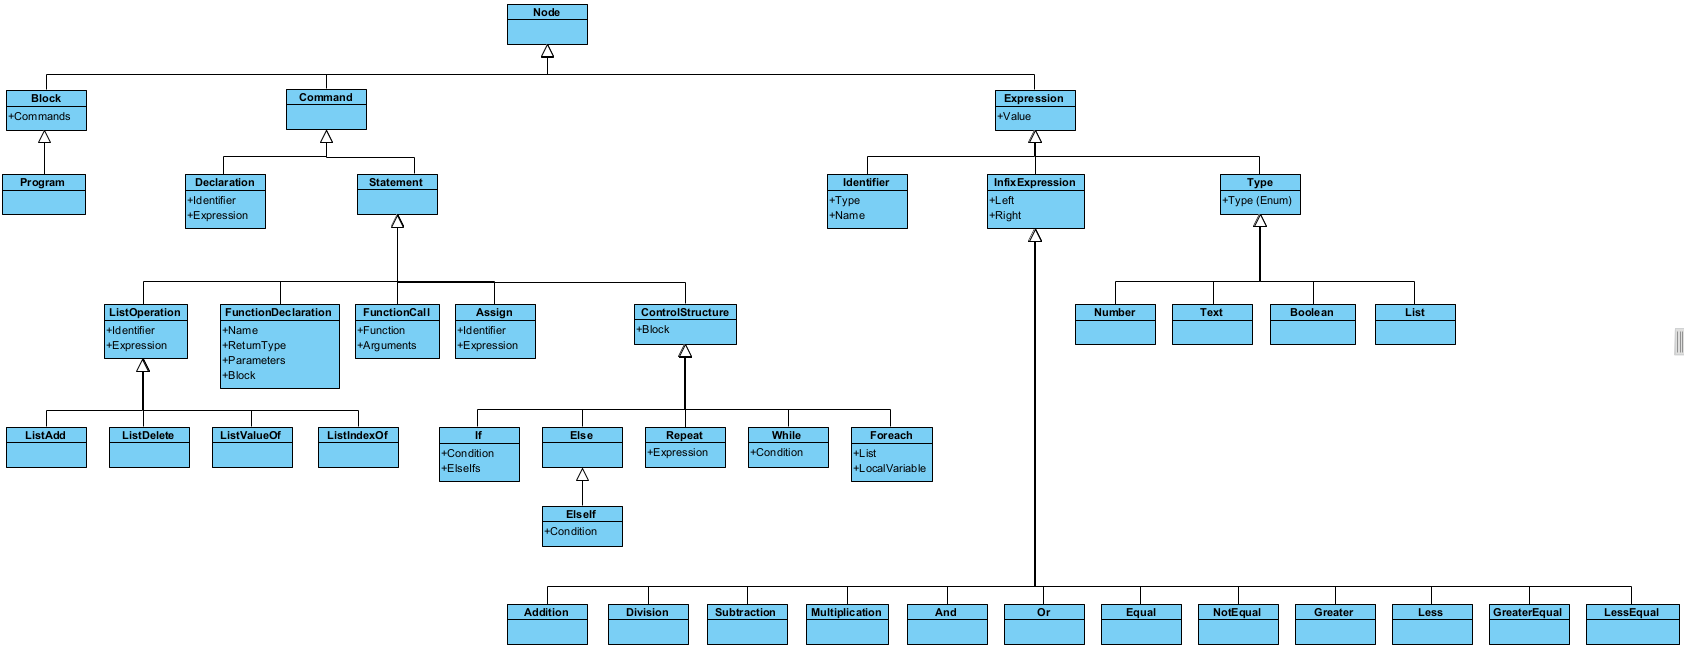
\includegraphics[width=1.5\textwidth, angle=90]{Files/Billeder: Design/ASTNodes.png}
    \end{center}
    \caption{The AST nodes in \lang represented as a class-diagram.}
    \label{ASTNodes}
\end{figure}
